\chapter{\uppercase{System Design}}
\label{ch:chap3}

\section{\uppercase{Design Principles}}
AgentOS is designed as a modular runtime. The gateway handles external requests, the orchestrator converts a prompt into a structured plan, and the kernel owns execution concerns. Redis is used for low-latency coordination and event transport, while MongoDB stores task history. ChromaDB stores embeddings used for semantic agent retrieval and context swap. The design keeps the current dependency truth in the DAG executor and treats scheduler decisions as admission and dispatch decisions.

\section{\uppercase{Overall Architecture}}
As shown in Figure~\ref{fig:architecture}, AgentOS is organised as an overall runtime architecture connecting the user interface, gateway, planner, kernel, storage, tools, agents, and model engines. The figure combines implemented runtime components with architectural modules that are planned or only partially implemented; their implementation status is documented separately in Section~\ref{sec:implementation-status}. A user submits a task through the Next.js interface. The FastAPI gateway creates or retrieves task state and communicates with the kernel. The planner selects agents and creates steps; the kernel validates and executes those steps while publishing activity events.
\begin{landscape}
\begin{figure}[p]
\centering
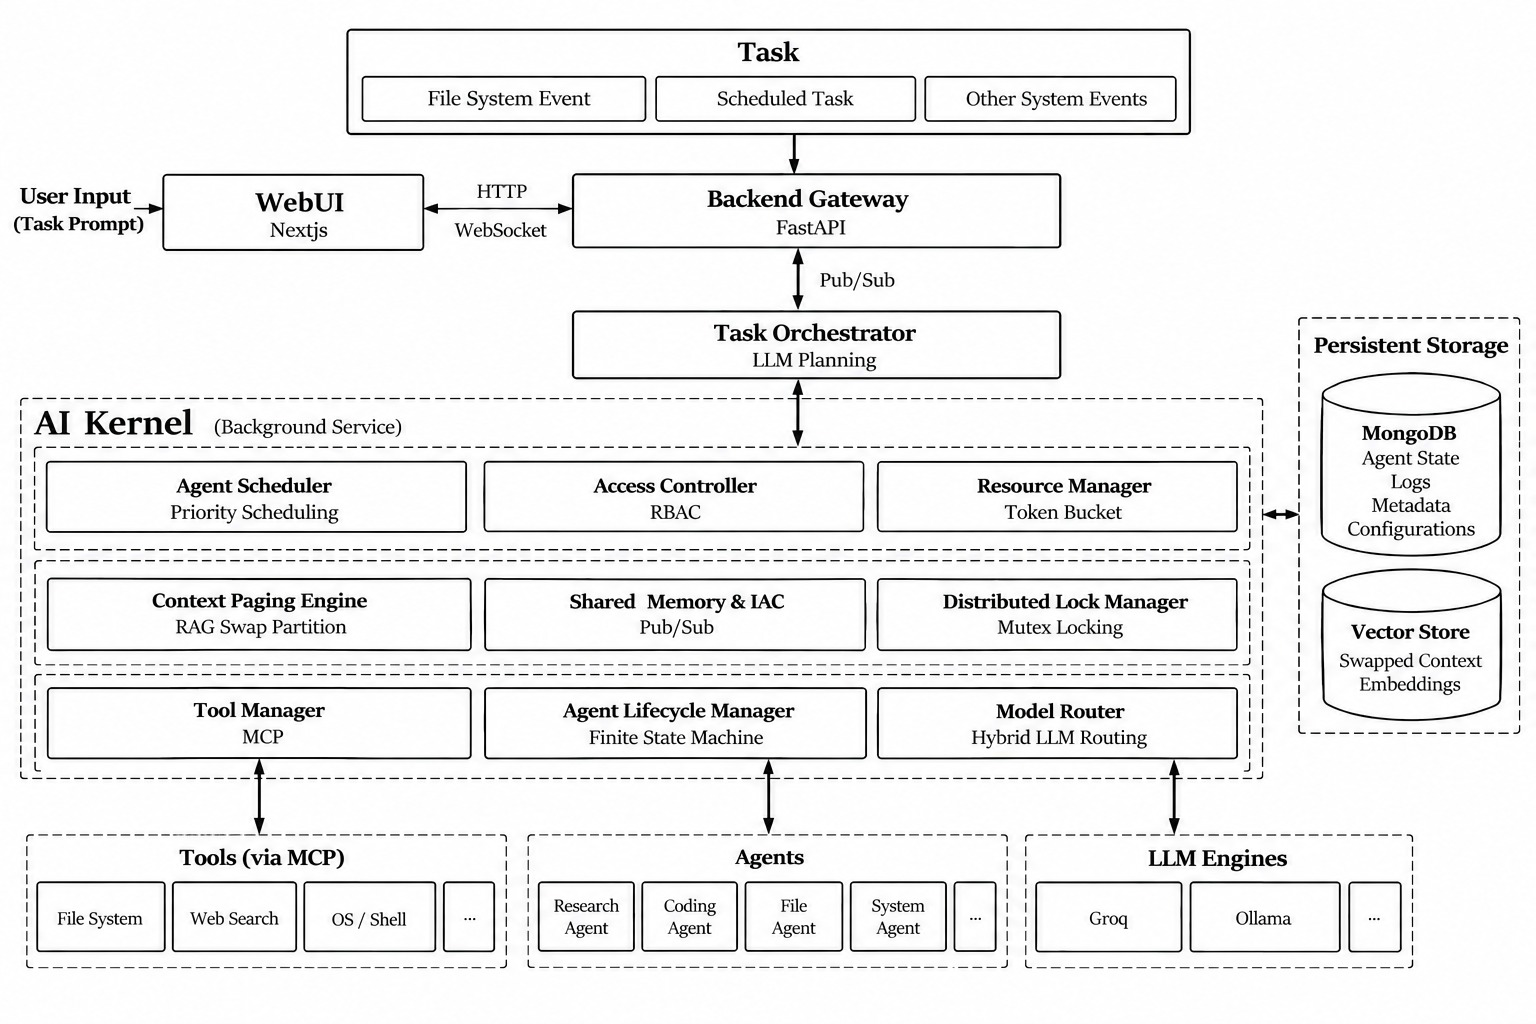
\includegraphics[width=0.99\linewidth,height=0.80\textheight,keepaspectratio]{3/figures/agentos_architecture.jpeg}
\caption{Overall AgentOS system architecture}
\label{fig:architecture}
\end{figure}
\end{landscape}

\section{\uppercase{Frontend, Gateway, and Event Flow}}
The frontend sends task prompts over HTTP and receives live activity over WebSocket. The backend listener subscribes to the kernel event channel and forwards events to connected clients. Figure~\ref{fig:redisflow} shows the separation between the task submission channel and the kernel event channel. MongoDB persistence is performed by the kernel/repository layer so the UI can later query task history.
\begin{figure}[H]
\centering
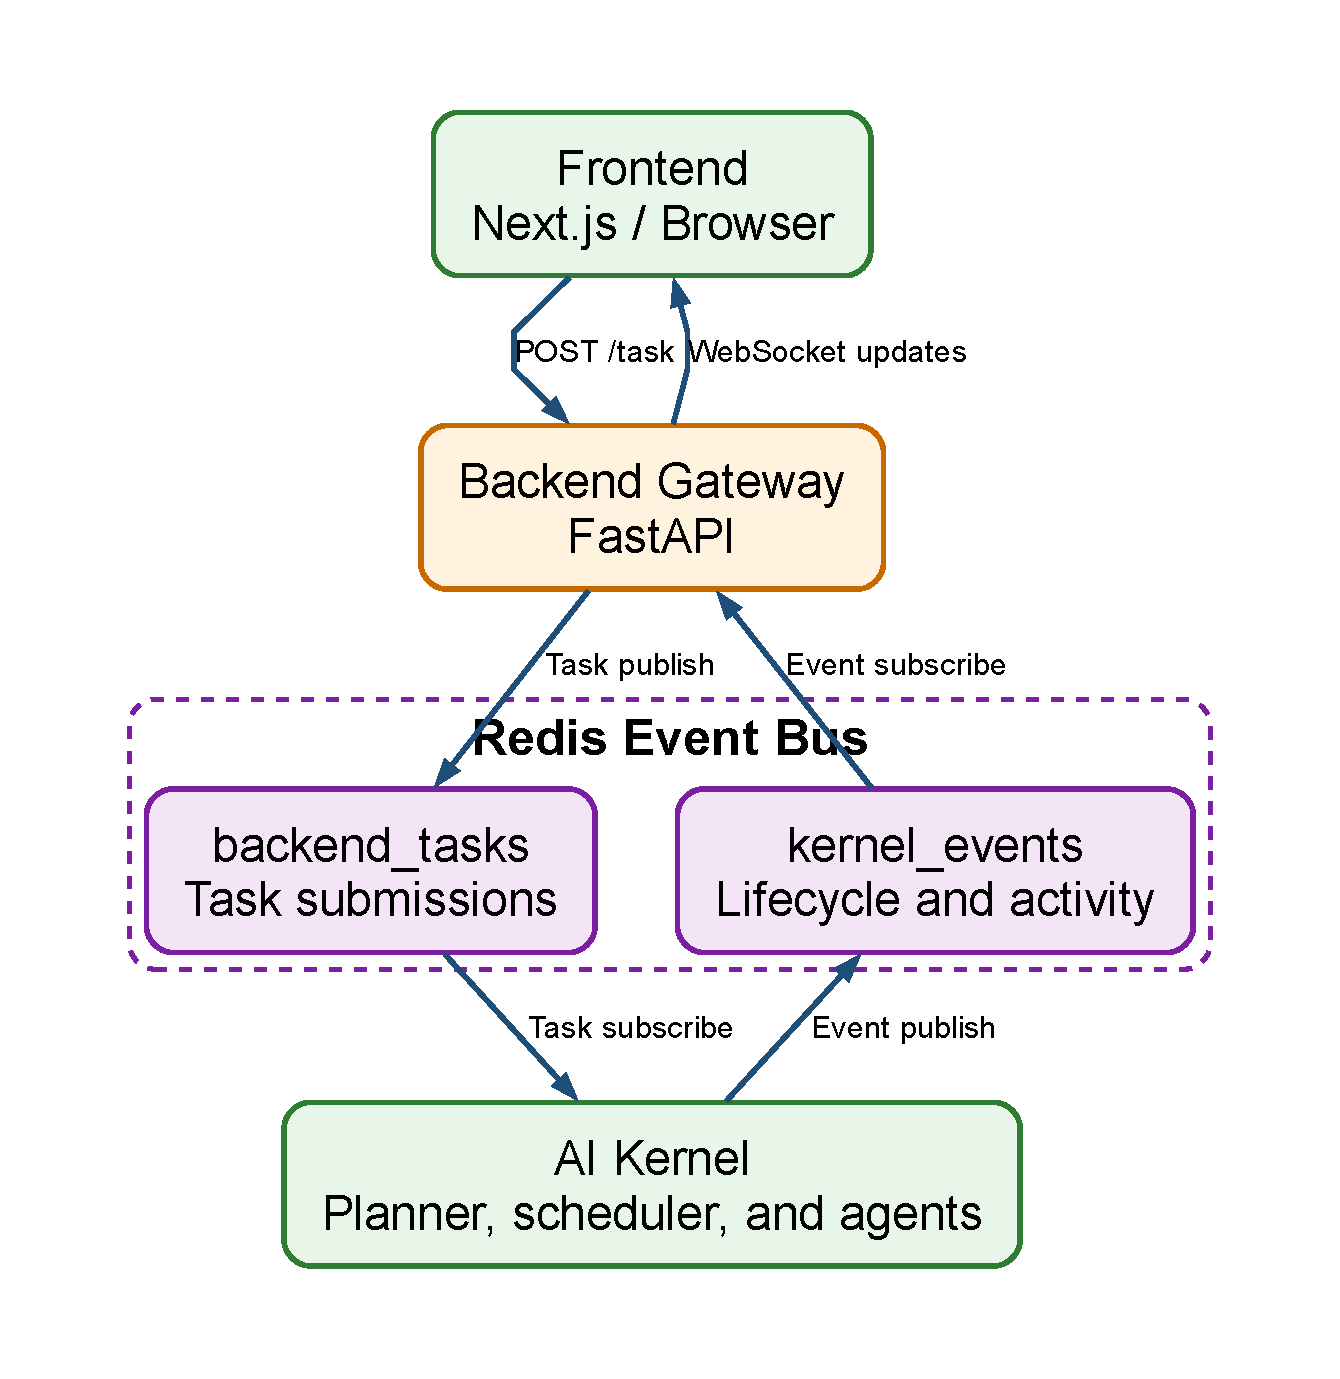
\includegraphics[width=1.0\textwidth,height=0.62\textheight,keepaspectratio]{3/figures/redis-flow-readable.pdf}
\caption{Frontend, FastAPI gateway, Redis channels, AI kernel, and agent-workforce flow}
\label{fig:redisflow}
\end{figure}

\section{\uppercase{Planner and DAG Execution}}
The planner retrieves relevant agent descriptions, requests a structured execution plan, and applies a fallback plan when the provider is unavailable. Each step includes an identifier, agent name, description, and dependency list. The validator canonicalises identifiers, rejects unknown dependencies and cycles, and supplies a sequential fallback only when a plan omits dependencies. The executor runs only steps whose prerequisites are complete. Figure~\ref{fig:dag} summarises this path. The frontend uses the same validated plan to generate Mermaid source and draw the plan graph, ensuring that displayed edges represent dependencies rather than decorative links.
\begin{figure}[H]
\centering
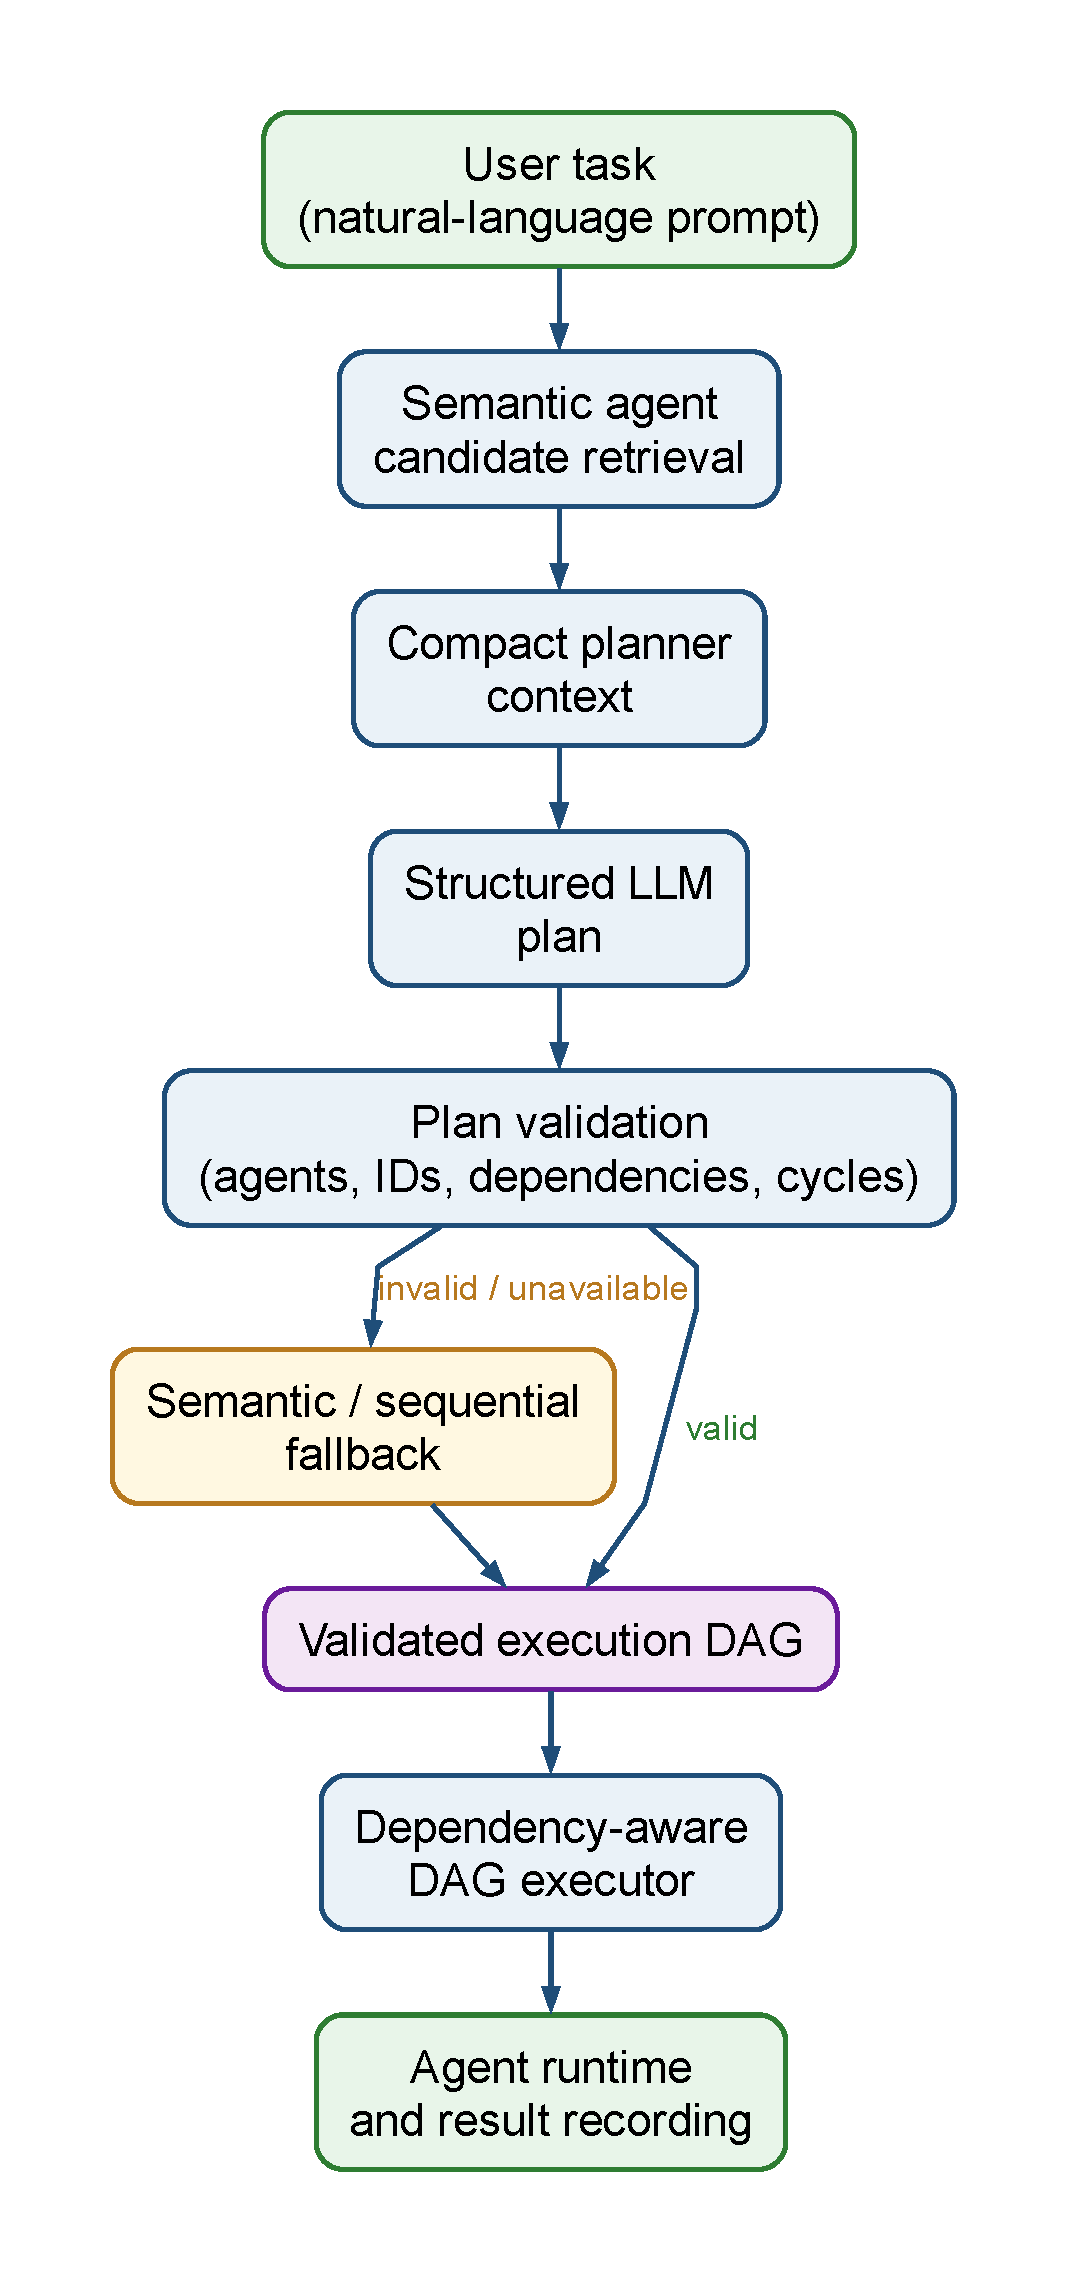
\includegraphics[width=0.90\textwidth,height=0.58\textheight,keepaspectratio]{3/figures/dag-readable.pdf}
\caption{Planner, validation, and dependency-aware execution flow}
\label{fig:dag}
\end{figure}

\clearpage
\section{\uppercase{Context Paging}}
The context pager keeps a bounded active message window. When the window is exceeded, older or less relevant messages are embedded and stored in the ChromaDB swap collection. A later query retrieves semantically related pages and injects them into the active context. ChromaDB's cosine space returns distance; the implementation converts it as $s=1-d$, where $d$ is the returned cosine distance. Figure~\ref{fig:context} presents the page-out and page-in flow. This mechanism reduces active prompt growth but does not guarantee perfect recall.
\begin{figure}[H]
\centering
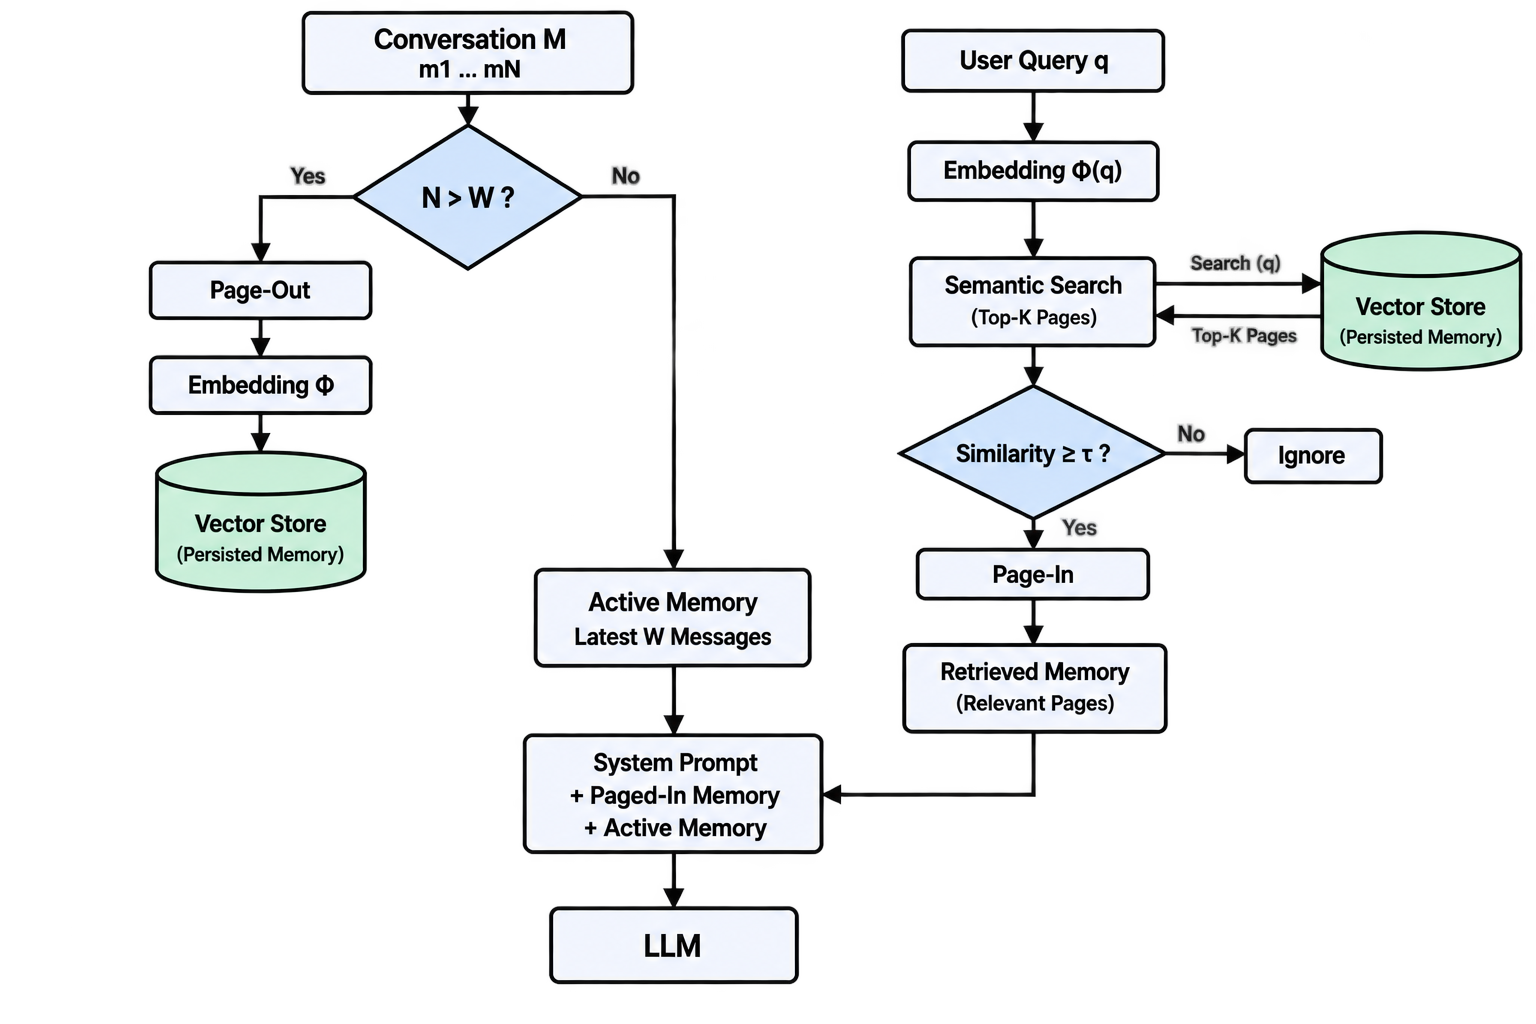
\includegraphics[width=1.0\textwidth]{3/figures/context_paging.png}
\caption{Context page-out, vector-store retrieval, and semantic page-in flow}
\label{fig:context}
\end{figure}

\section{\uppercase{Global Scheduler and Resource Manager}}
The scheduler maintains ready records and selects work globally across active tasks. Effective priority is computed from base priority and queue waiting time, bounded by a maximum. Before dispatch, the resource manager checks the global slot limit, per-task slot limit, and token budget. The current defaults are three global execution slots, two slots per task, and a configurable 50,000-token task budget. Dispatch is cooperative: a running remote LLM request is not forcibly killed. Figure~\ref{fig:scheduler} shows the decision path.
\begin{figure}[H]
\centering
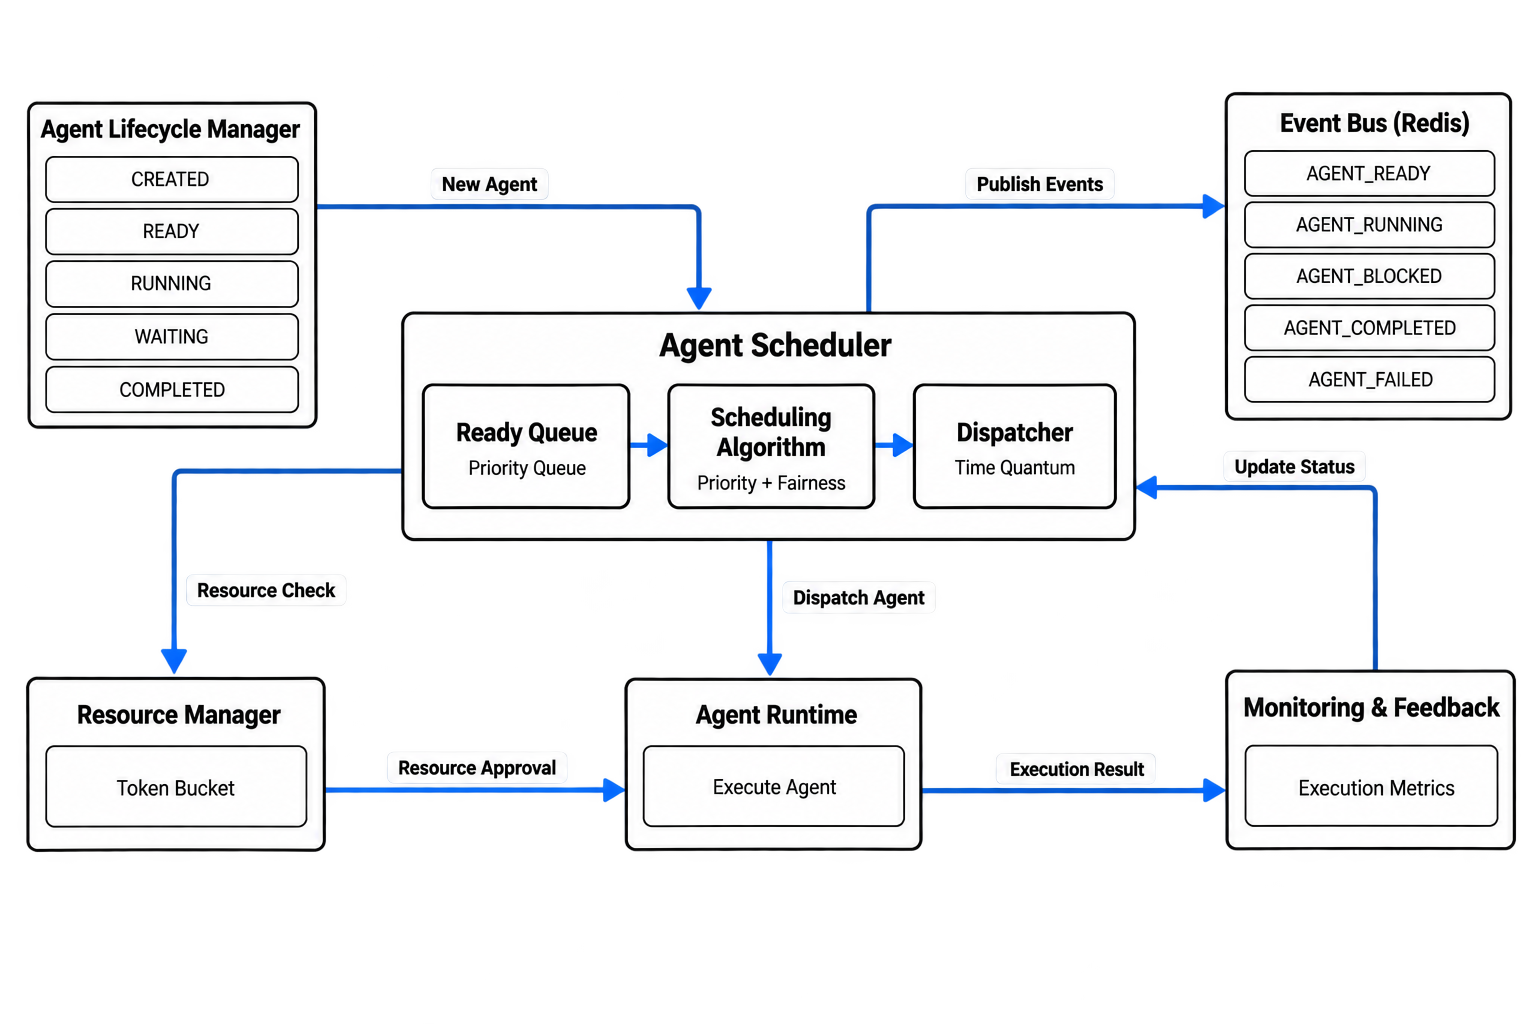
\includegraphics[width=1.0\textwidth]{3/figures/agent_scheduler.png}
\caption{Global agent scheduler, lifecycle events, resource checks, and runtime feedback}
\label{fig:scheduler}
\end{figure}

\section{\uppercase{Resource Management}}
The resource-manager design in Figure~\ref{fig:resource-manager} expands the admission point in the scheduler. It separates token-bucket accounting, quota monitoring, process monitoring, resource checking, and the final decision. In the current implementation, the corresponding resource manager enforces global and per-task execution slots and a token budget; the policy store, process monitor, and hard preemption shown in the figure are design extensions.
\begin{figure}[H]
\centering
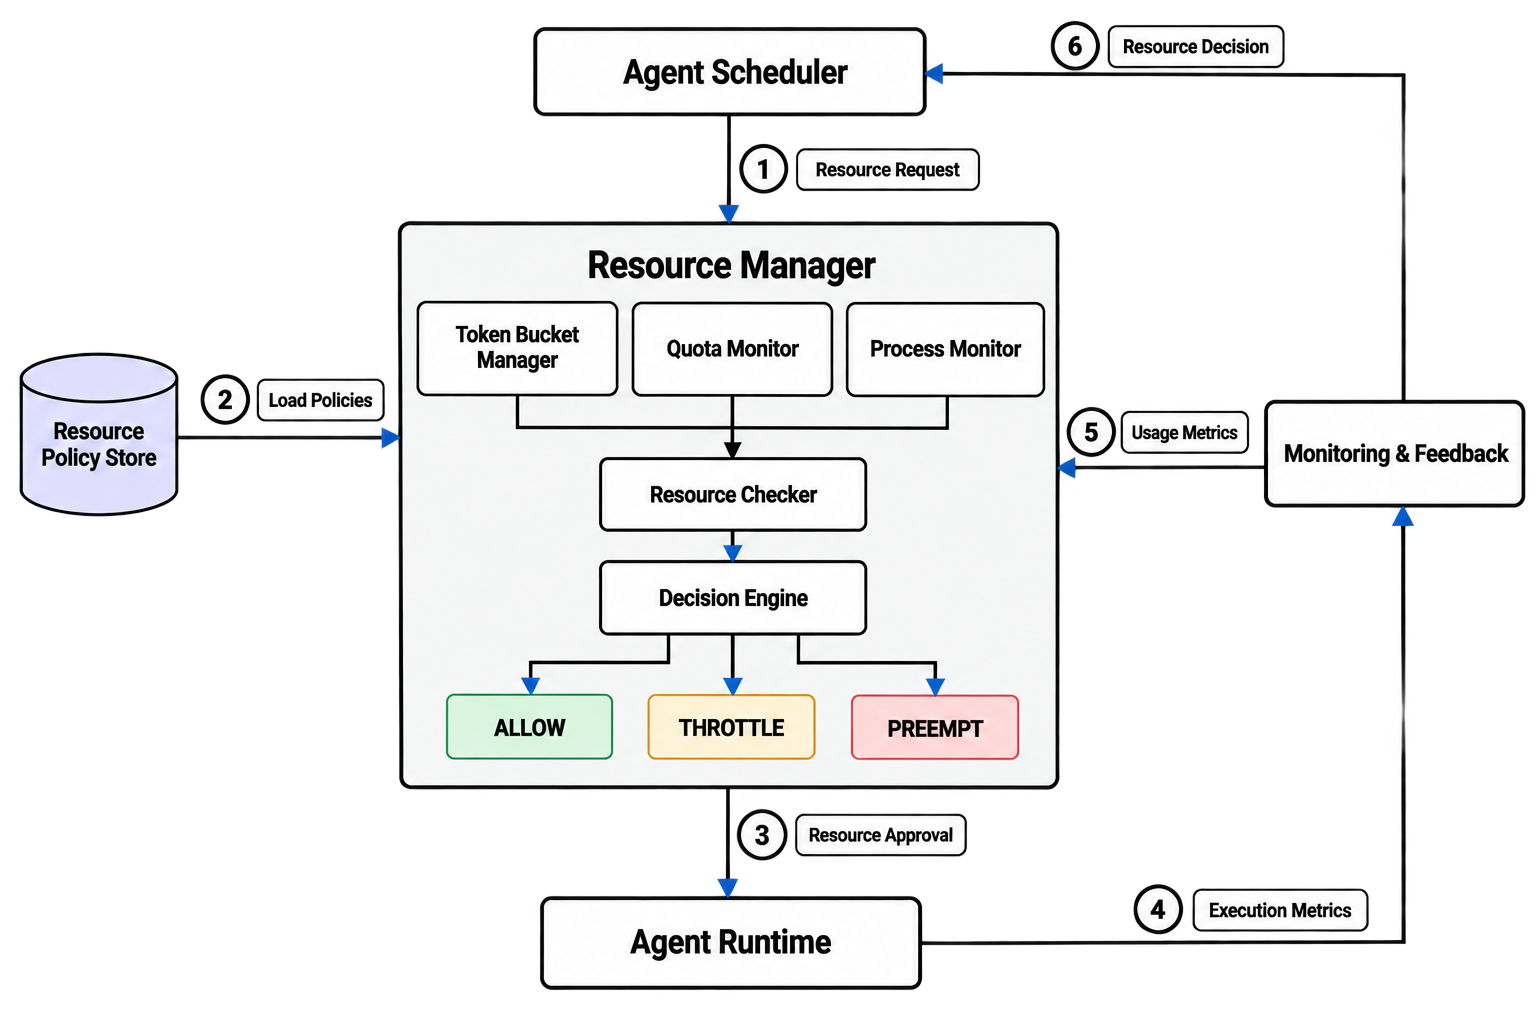
\includegraphics[width=1.0\textwidth]{3/figures/resource_manager.png}
\caption{Resource-manager decision flow supplied for the AgentOS design}
\label{fig:resource-manager}
\end{figure}

\section{\uppercase{Tool Management}}
Figure~\ref{fig:tool-manager} shows the intended tool-manager boundary between an agent, a tool registry, permission policy, and local or external services. AgentOS currently exposes bounded tools through the runtime and code runner; a complete permission store and MCP-compatible tool manager remain proposed components.
\begin{figure}[H]
\centering
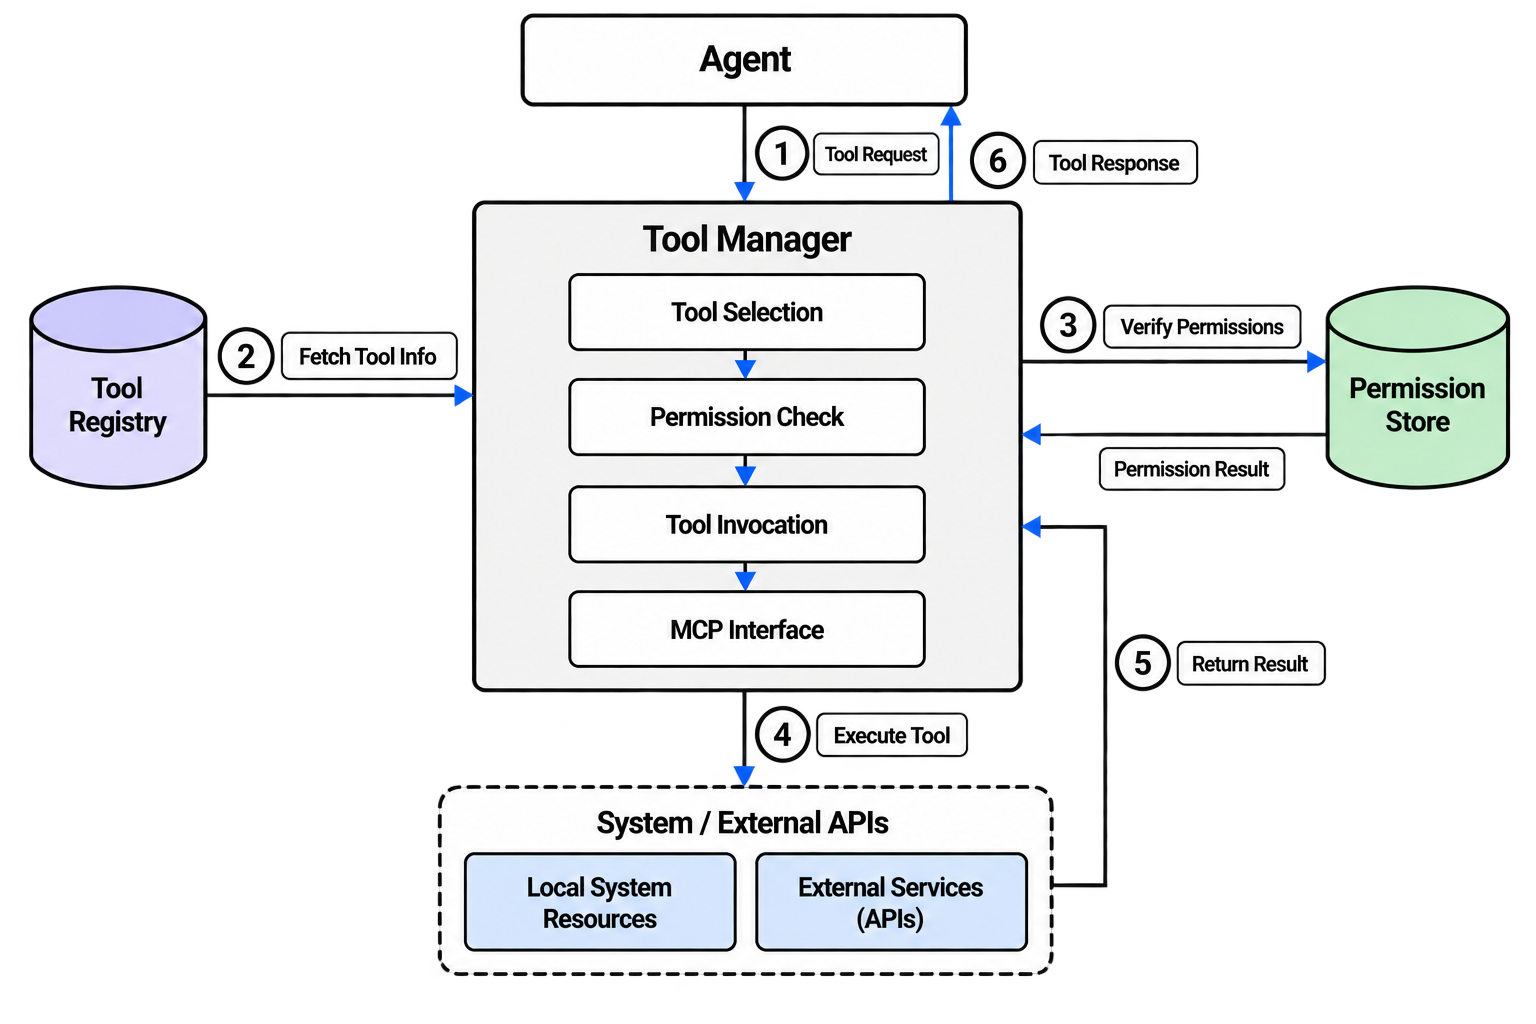
\includegraphics[width=1.0\textwidth]{3/figures/tool_manager.png}
\caption{Tool selection, permission checking, invocation, and result return}
\label{fig:tool-manager}
\end{figure}

\section{\uppercase{Agent Lifecycle and Events}}
An agent step progresses from CREATED to READY, RUNNING, and COMPLETED. It can move to WAITING when a resource or dependency is unavailable, or to BLOCKED/FAILED when execution cannot proceed. The scheduler and runtime publish structured lifecycle events containing task, step, agent, execution, status, priority, queue wait, and attempt information. Figure~\ref{fig:lifecycle} shows the state model. RBAC, distributed mutex locking, and complete state-machine enforcement are architectural extensions rather than claims of full implementation in this phase.
\begin{figure}[H]
\centering
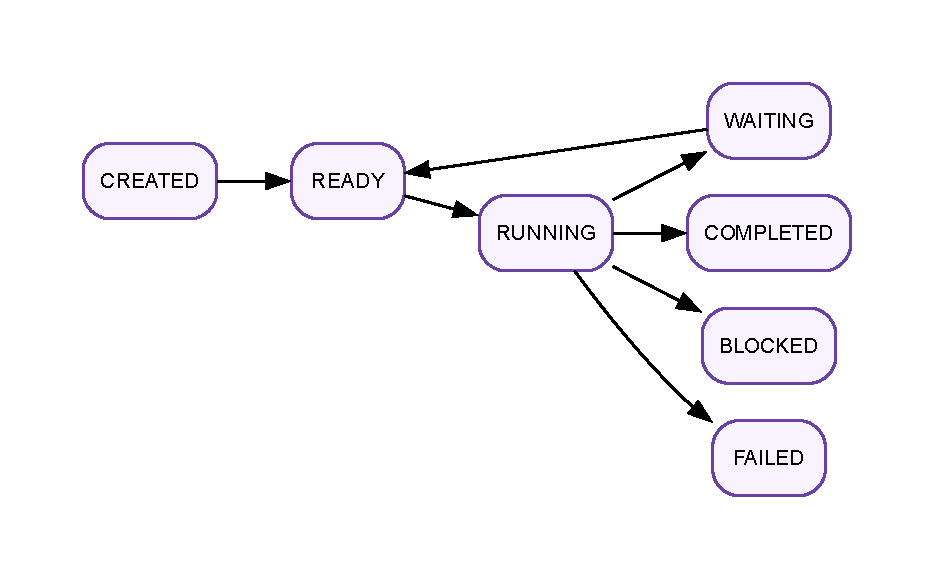
\includegraphics[width=0.9\textwidth]{3/figures/lifecycle.pdf}
\caption{Agent lifecycle transitions}
\label{fig:lifecycle}
\end{figure}

\section{\uppercase{Sandboxed Code Runner}}
The code runner receives generated Python, writes it into a scoped working directory, and invokes it through an asynchronous subprocess. It bounds execution time and captured output. A non-zero exit code or traceback is returned to the coder/tester agent, which may produce a corrected version for at most three attempts. Output lines can be published as kernel events for live frontend observation. Figure~\ref{fig:runner} shows this flow. The current isolation is process and directory scoping; hardened container or microVM isolation is future work.
\begin{figure}[H]
\centering
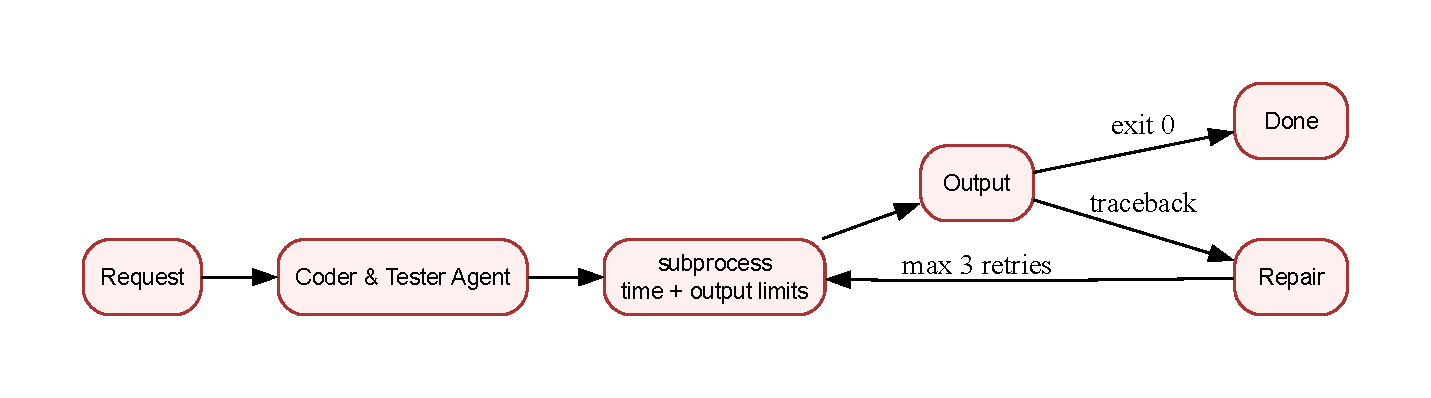
\includegraphics[trim=0.7cm 0.7cm 0.7cm 0.7cm,clip,width=1.0\textwidth,height=0.82\textheight,keepaspectratio]{3/figures/runner.pdf}
\caption{Sandboxed Python execution and bounded self-healing loop}
\label{fig:runner}
\end{figure}

\section{\uppercase{Implemented and Proposed Boundaries}}
\label{sec:implementation-status}
Table~\ref{tab:boundary} records the design boundary used throughout the report.
\begin{table}[H]
\centering
\caption{Implemented and future AgentOS modules}
\label{tab:boundary}
\begin{tabular}{>{\raggedright\arraybackslash}p{4.2cm}p{5.3cm}p{4.2cm}}
\toprule
Module & Current implementation & Status / limitation \\
\midrule
Frontend and gateway & Next.js, FastAPI, WebSocket activity & Implemented \\
Planner and DAG & Structured plan, validation, Mermaid graph & Implemented \\
Scheduler and resources & Priority aging, slots, token admission & Implemented; cooperative only \\
Context paging & ChromaDB semantic swap and retrieval & Implemented \\
Redis and MongoDB & Events, queue metadata, task history & Implemented \\
Code runner & Bounded Python subprocess and retries & Implemented; not microVM isolation \\
RBAC / capability policy & Architecture documented & Proposed \\
Distributed locks / workers & Architecture documented & Future \\
Hybrid model routing & Provider abstraction is partial & Future \\
Durable coroutine restoration & Interrupted records are detected/requeued policy is partial & Future \\
\bottomrule
\end{tabular}
\end{table}
